%Author Sujeendra R
\documentclass[12pt]{article}

\usepackage{fancybox}%for border and many more packages are not used

\usepackage{subfig}
\usepackage{wrapfig}
\usepackage{wasysym}
\usepackage{enumitem}
\usepackage{adjustbox}
\usepackage{ragged2e}    %packages imported which are required 
\usepackage[svgnames,table]{xcolor}
\usepackage{tikz}
\usepackage{longtable}
\usepackage{changepage}
\usepackage{setspace}
\usepackage{hhline}
\usepackage{multicol}
\usepackage{tabto}
\usepackage{float}
\usepackage{multirow}
\usepackage{makecell}
\usepackage{fancyhdr}
\usepackage[toc,page]{appendix}
\usepackage[hidelinks]{hyperref}
\usetikzlibrary{shapes.symbols,shapes.geometric,shadows,arrows.meta}
\tikzset{>={Latex[width=1.5mm,length=2mm]}}
\usepackage{flowchart}\usepackage[paperheight=11.69in,paperwidth=8.27in,left=0.98in,right=0.98in,top=0.98in,bottom=0.98in,headheight=1in]{geometry}
\usepackage[utf8]{inputenc}
\usepackage[T1]{fontenc}
\TabPositions{0.49in,0.98in,1.47in,1.96in,2.45in,2.94in,3.43in,3.92in,4.41in,4.9in,5.39in,5.88in,}

\urlstyle{same}

\setcounter{tocdepth}{5}
\setcounter{secnumdepth}{5}
 %setting boundry condition and margin parameters which are preset in ms word
\setlistdepth{9}
\renewlist{enumerate}{enumerate}{9}
		\setlist[enumerate,1]{label=\arabic*)}
		\setlist[enumerate,2]{label=\alph*)}
		\setlist[enumerate,3]{label=(\roman*)}
		\setlist[enumerate,4]{label=(\arabic*)}
		\setlist[enumerate,5]{label=(\Alph*)}
		\setlist[enumerate,6]{label=(\Roman*)}
		\setlist[enumerate,7]{label=\arabic*}
		\setlist[enumerate,8]{label=\alph*}
		\setlist[enumerate,9]{label=\roman*}

\renewlist{itemize}{itemize}{9}
		\setlist[itemize]{label=$\cdot$}
		\setlist[itemize,1]{label=\textbullet}
		\setlist[itemize,2]{label=$\circ$}
		\setlist[itemize,3]{label=$\ast$}
		\setlist[itemize,4]{label=$\dagger$}
		\setlist[itemize,5]{label=$\triangleright$}
		\setlist[itemize,6]{label=$\bigstar$}
		\setlist[itemize,7]{label=$\blacklozenge$}
		\setlist[itemize,8]{label=$\prime$}

\setlength{\topsep}{0pt}\setlength{\parindent}{0pt}
\renewcommand{\arraystretch}{1.3}





%start of the document
\begin{document}
%naming
\begin{Center}
{\fontsize{16pt}{19.2pt}\selectfont  \textbf{ SUJEENDRA\ R\ \   }{\fontsize{13pt}{15.6pt}\selectfont \textbf{\ \ \ \ \ \ \ \ \ \ \  }\par}\par}\par

\end{Center}


%image path must be specified
\begin{figure}[H]
	\begin{FlushRight}		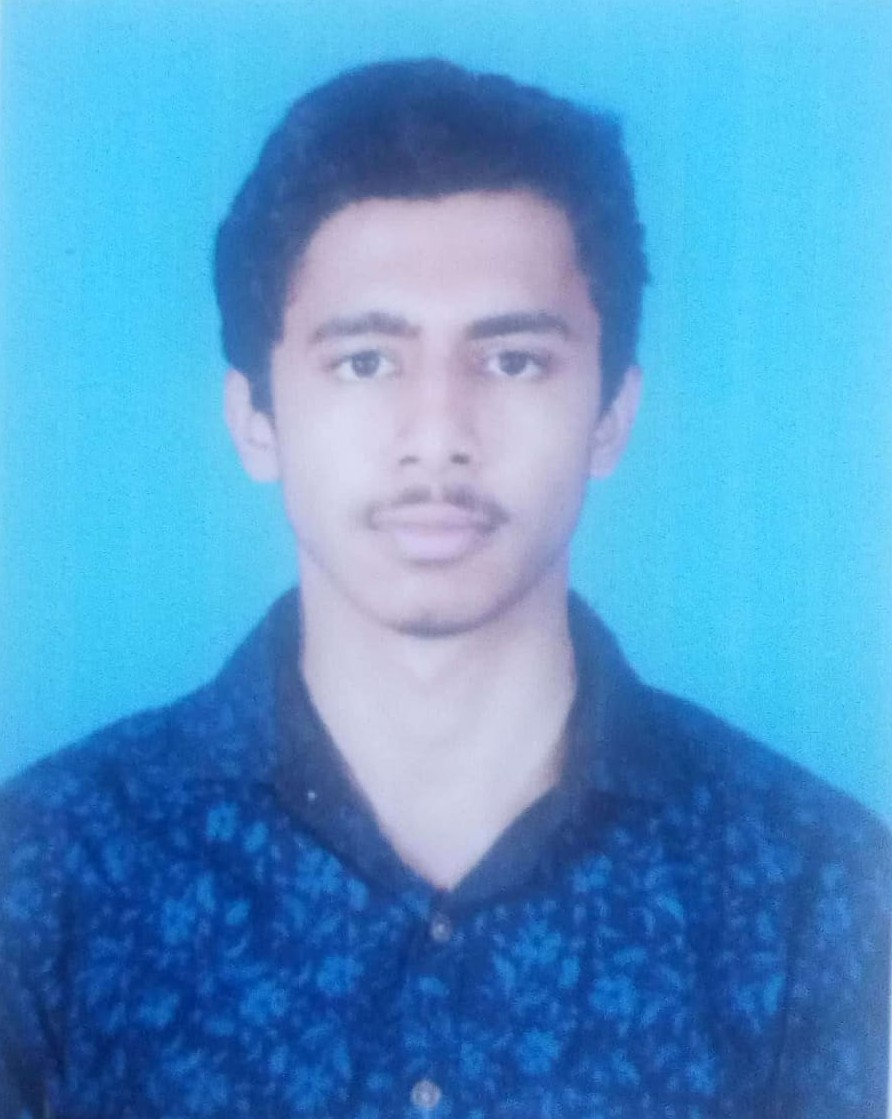
\includegraphics[width=1.08in,height=1.44in]{/home/sujeendra/Documents/Sujeendra_R_resume/Profile.jpeg}
	\end{FlushRight}\end{figure}



%address
\vspace{-4.2cm}

{\fontsize{13pt}{15.6pt}\selectfont \textbf{$\#$ 31 4\textsuperscript{th} A main CITB model}\par}\par

{\fontsize{13pt}{15.6pt}\selectfont \textbf{House Near Library Subhash Nagar}\par}\par

{\fontsize{13pt}{15.6pt}\selectfont \textbf{Karnataka Mysore-570007}\par}\par

{\fontsize{13pt}{15.6pt}\selectfont \textbf{Contact:7026335428}\par}\par

{\fontsize{13pt}{15.6pt}\selectfont \textbf{email id: sujeendrar.280@gmail.com}\par}


\vspace{\baselineskip}

\vspace{\baselineskip}

%objective
\vspace{\baselineskip}
{\fontsize{14pt}{16.8pt}\selectfont \textbf{Objective}\par}\par

{\fontsize{13pt}{15.6pt}\selectfont I have a keen interset in learning new topics ,so i would like to work on more Technical Projects like Eyantra ,especially on a subject like Robotics and Computer Vision.\par}\par


%for spacing between lines
\vspace{\baselineskip}
{\fontsize{14pt}{16.8pt}\selectfont \textbf{Education}\par}\par





%Education
\begin{table}[H]
 			\centering
\begin{tabular}{p{1.37in}p{1.37in}p{1.37in}p{1.38in}}
\hline
%1
\multicolumn{1}{|p{1.37in}}{\begin{Center}Degree\end{Center}} & 
\multicolumn{1}{|p{1.37in}}{\begin{Center}College/School\end{Center}} & 
\multicolumn{1}{|p{1.37in}}{\begin{Center}Passing Year\end{Center}} & 
\multicolumn{1}{|p{1.38in}|}{\begin{Center}Percentage\end{Center}} \\
\hhline{----}
%2
\multicolumn{1}{|p{1.37in}}{\begin{Center}SSLC\end{Center}} & 
\multicolumn{1}{|p{1.37in}}{\begin{Center}Marimallappa’s High School Mysore\end{Center}} & 
\multicolumn{1}{|p{1.37in}}{\begin{Center}2014\end{Center}} & 
\multicolumn{1}{|p{1.38in}|}{\begin{Center}97.44\end{Center}} \\
\hhline{----}
%3
\multicolumn{1}{|p{1.37in}}{\begin{Center}PUC\end{Center}} & 
\multicolumn{1}{|p{1.37in}}{\begin{Center}Marimallappa’s PU College Mysore\end{Center}} & 
\multicolumn{1}{|p{1.37in}}{\begin{Center}2016\end{Center}} & 
\multicolumn{1}{|p{1.38in}|}{\begin{Center}94\end{Center}} \\
\hhline{----}
%4
\multicolumn{1}{|p{1.37in}}{\begin{Center}B.E in Electronics and Communication\end{Center}} & 
\multicolumn{1}{|p{1.37in}}{\begin{Center}Sri Jayachamarajendra College of Enginnering(JSSTU)\end{Center}} & 
\multicolumn{1}{|p{1.37in}}{\begin{Center}2020\end{Center}} & 
\multicolumn{1}{|p{1.38in}|}{\begin{Center}CGPA on a scale of 10 .Five semester Score is\end{Center} \begin{Center}\par 9.3 \end{Center}\par } \\
\hhline{----}

\end{tabular}
 \end{table}
 
 
 %projects
\vspace{0.1cm}
{\fontsize{14pt}{16.8pt}\selectfont \textbf{Projects}\par}\par


\vspace{0.1cm}
\begin{enumerate}[label*={\fontsize{13pt}{13pt}\selectfont \textbf{\textbf{\arabic*.}}}]
	\item {\fontsize{13pt}{15.6pt}\selectfont \textbf{Chatbot-using-Raspberry-pi-For-Building-Navigation}\par}\par

\begin{enumerate}
	\item {\fontsize{13pt}{15.6pt}\selectfont \textbf{Description}: Chatbot using Raspberry-pi to navigate inside the building or apartment Using TCP Protocol.\par}\par

	\item {\fontsize{13pt}{15.6pt}\selectfont \textbf{Link}: \href{https://github.com/Sujeendra/Chatbot-using-Raspberry-pi-For-Building-Navigation}{https://github.com/Sujeendra/Chatbot-using-Raspberry-pi-For-Building-Navigation} \par}\end{enumerate}\par


\vspace{0.1cm}
	\item {\fontsize{13pt}{15.6pt}\selectfont \textbf{Google-Home-Prototype-using-RPI-3B}\par}\par
\begin{enumerate}
	\item {\fontsize{13pt}{15.6pt}\selectfont \textbf{Description}: Google assiatnt will be installed on Raspberry pi and configured for .asoundrc file for setting up USB mic which act as an an voice input device for controlling any gadget via voice commands.\par}\par

	\item {\fontsize{13pt}{15.6pt}\selectfont \textbf{Link}: \href{https://github.com/Sujeendra/Google-Home-Prototype-using-RPI-3B}{https://github.com/Sujeendra/Google-Home-Prototype-using-RPI-3B}\par}\end{enumerate}\par


\vspace{\baselineskip}
	\item {\fontsize{13pt}{15.6pt}\selectfont \textbf{OpenCV-Projects-based-on-Facial-recognition}\par}\par
\begin{enumerate}
	\item {\fontsize{13pt}{15.6pt}\selectfont \textbf{Description}: This project uses lbhp i.e. linear binary histogram patterns to match faces wih dataset and also python speech recoognition is used to check whether user is an admin or someother person.\par}\par

	\item {\fontsize{13pt}{15.6pt}\selectfont \textbf{link}: \href{https://github.com/Sujeendra/OpenCV-3.4-Projects-based-on-Fcaial-recognition-and-Python-Speech-recognition}{https://github.com/Sujeendra/OpenCV-3.4-Projects-based-on-Fcaial\\-recognition-and-Python-Speech-recognition}\par}\end{enumerate}\par


\vspace{0.01cm}

\vspace{0.1cm}
	\item {\fontsize{13pt}{15.6pt}\selectfont \textbf{Interfacing-LED-with-Raspberry-Pi-3B}\par}\par
\begin{enumerate}
	\item {\fontsize{13pt}{15.6pt}\selectfont \textbf{Description}: A simple Incrementer code is written using python to display counting action til 60seconds on Common Cathode Led Connected to Pi using GPIO pins.\par}\par

	\item {\fontsize{13pt}{15.6pt}\selectfont \textbf{link}: \href{https://github.com/Sujeendra/Interfacing-LED-with-Raspberry-Pi-3B}{https://github.com/Sujeendra/Interfacing-LED-with-Raspberry-Pi-3B}\par}\end{enumerate}\par


\vspace{0.1cm}
	\item {\fontsize{13pt}{15.6pt}\selectfont \textbf{Tic tac Toe game using Android studio }\par}

\begin{enumerate}
	\item {\fontsize{13pt}{15.6pt}\selectfont \textbf{Description}: A simple android app Developed using android studio using Java programming Language.\par}\par

	\item {\fontsize{13pt}{15.6pt}\selectfont \textbf{link}: \href{https://github.com/Sujeendra/Tic-tac-toe-Game-using-Android-Studio-and-Java}{https://github.com/Sujeendra/Tic-tac-toe-Game-using-Android-Studio-and-Java}\par}\end{enumerate}\par


\vspace{0.1cm}
{\fontsize{13pt}{15.6pt}\selectfont Other projects: Automatic Bidirectional Person counter using Arduino Uno and DTMF controlled Appliances. Also Eyantra-2018 was my biggest Project among all.\par}\end{enumerate}\par


%Internship
\vspace{\baselineskip}


{\fontsize{14pt}{16.8pt}\selectfont \textbf{Internship}\par}\par
\begin{itemize}
\item{\fontsize{13pt}{15.6pt}\selectfont \textbf{Sanfoundry: }Content Writing Mcq’s$ \vert $  Topic : Engineering Mathematics.\par}\par

{\fontsize{13pt}{15.6pt}\selectfont Duartion: October 2017 to Decemeber 2017\par}\par

\item{\fontsize{13pt}{15.6pt}\selectfont \textbf{Grade Up:}Content\ Writing  $ \vert $  JEE/IIT Exam Mcq’s $ \vert $  Topic : Mathematics.\par}\par

{\fontsize{13pt}{15.6pt}\selectfont Duartion : October 2017 to May 2018\par}\par

\item{\fontsize{13pt}{15.6pt}\selectfont \textbf{Unacadamy: }Created Mathematics Tutorial Videos for IIT/JEE examination.\par}\par

{\fontsize{13pt}{15.6pt}\selectfont Duration: June 2018 to July 2018\par}\par
\end{itemize}


%Technical skills
\vspace{4cm}
{\fontsize{14pt}{16.8pt}\selectfont \textbf{Technical Skills}\par}\par

\begin{enumerate}
	\item {\fontsize{13pt}{15.6pt}\selectfont Programming and coding\par}\par
\begin{enumerate}

	\item {\fontsize{13pt}{15.6pt}\selectfont C-Programming \par}\par

	\item {\fontsize{13pt}{15.6pt}\selectfont  Java\par}\par

	\item {\fontsize{13pt}{15.6pt}\selectfont  Python\par}\par

	\item {\fontsize{13pt}{15.6pt}\selectfont  Data Structures using C++\par}\end{enumerate}\par

	\item {\fontsize{13pt}{15.6pt}\selectfont Matlab\par}\par

	\item {\fontsize{13pt}{15.6pt}\selectfont ROS-Robot Operating System and Vrep Software\par}\par

	\item {\fontsize{13pt}{15.6pt}\selectfont Tina Ti Circuit Design\par}\par

	\item {\fontsize{13pt}{15.6pt}\selectfont Python Open CV\par}\par
	\item {\fontsize{13pt}{15.6pt}\selectfont Linux(Ubuntu)\par}\par
	\item {\fontsize{13pt}{15.6pt}\selectfont Android Studio Development Basic\par}\par

	\item {\fontsize{13pt}{15.6pt}\selectfont Reporting Software Bugs in Custom Roms for my device k5fpr(Lenovo Vibe K4 note) on XDA Platform\par}\par

	\item {\fontsize{13pt}{15.6pt}\selectfont 8051 Microcontroller Assembly level Programming\par}\par

	\item {\fontsize{13pt}{15.6pt}\selectfont Ardunio Uno C programming\par}\par

	\item {\fontsize{13pt}{15.6pt}\selectfont Creating\ \ Basic Videos  using slides.\par}\par

	\item {\fontsize{13pt}{15.6pt}\selectfont Content Writing\par}
\end{enumerate}\par

%Soft skills
\vspace{0.1cm}
{\fontsize{14pt}{16.8pt}\selectfont \textbf{Soft Skills}\par}\par


\begin{itemize}
	\item {\fontsize{13pt}{15.6pt}\selectfont Communication Skills\par}\par

	\item {\fontsize{13pt}{15.6pt}\selectfont Responsibility\par}\par

	\item {\fontsize{13pt}{15.6pt}\selectfont Ability to Work under Pressure\par}\par

	\item {\fontsize{13pt}{15.6pt}\selectfont Team Work\par}
\par
\end{itemize}

%Co curricular activities
\vspace{0.1cm}
{\fontsize{14pt}{16.8pt}\selectfont \textbf{Co-Curricular Activities}\par}\par

\begin{enumerate}[label*={\fontsize{13pt}{13pt}\selectfont \arabic*.}]
	\item {\fontsize{13pt}{15.6pt}\selectfont Content Writing\par}\par
	\item {\fontsize{13pt}{15.6pt}\selectfont Flashing and Testing Custom Roms\par}
	\item {\fontsize{13pt}{15.6pt}\selectfont Coding on Hackerrank\par}
\end{enumerate}\par

%Extra Curricular

\vspace{1cm}
{\fontsize{14pt}{16.8pt}\selectfont \textbf{Extra Curricular Activities}\par}\par

\begin{itemize}
	\item {\fontsize{13pt}{15.6pt}\selectfont Drawing\par}\par
	\item {\fontsize{13pt}{15.6pt}\selectfont Sports\par}
	\item {\fontsize{13pt}{15.6pt}\selectfont Playing PC games\par}
\par
\end{itemize}

\end{document}